\documentclass[a4paper,12pt]{article}

\usepackage[in]{fullpage}
\usepackage{parskip}
\usepackage{tikz}
\usepackage[backend=bibtex,style=numeric-comp,sorting=nyt,sortcites=true]{biblatex}
\usepackage[section]{placeins}

\title{Qualifying Dissertation}
\author{James Baxter}
\date{}

\bibliography{literature} 

\newcommand{\Circus}{{\sffamily \slshape Circus}}

\begin{document}
\maketitle

\section{Introduction}

% need a short paragraph describing the structure of the Introduction

\subsection{Motivation}

Since its release in 1995, the Java programming language~\cite{gosling2013} has increased in popularity and is now used on a wide variety of platforms.
This popularity means that Java has been used in a wide variety of areas including desktop applications, on the internet in the form of Java applets, on smartcards~\cite{chen2000} and on mobile devices~\cite{oracle2014}.
Several languages derived from Java have also been created, including Scala~\cite{lausanne2015} and Ceylon~\cite{redhat2015}, as well as older variants of Java such as MultiJava~\cite{clifton2006} and Pizza~\cite{odersky1997}, which have in turn contributed to the development of Java.
% add a short sentence describing each langauage, try to find more non-webpage references

One use of Java that is of particular interest is its use in embedded systems.
While early versions of Java were developed with the intention of using them on embedded systems, particularly TV set-top boxes, the technology was not well received and it was only in the growing sector of the internet that Java intitially found a market. % need citation for this - horstmann2002?
However, it was soon realised that the portability, modularity, safety and security benefits of Java could be of great use in embedded systems. % need citation for this
This required the creation of specialised Java virtual machines as the standard JVM is too large for most embedded systems and much research has gone into making increasingly smaller virtual machines to increase the range of devices that Java can be used on~\cite{caska2011,thomm2010}.

Many embedded systems are also real-time systems, but features of Java such as the garbage collector and the concurrency model make it unsuitable for real-time systems, where strict guarantees about timing properties must be made.
To rectify these problems the Real-Time Specification for Java (RTSJ)~\cite{gosling2000} was created.
The RTSJ extends Java with a scoped memory model and a more predictable scheduling system, which allow RTSJ programs to fulfil real-time requirements.

While the RTSJ addresses real-time requirements of embedded systems, many embedded systems are also safety-critical.
Safety-critical programs must usually be shown to conform to certain standards of safety such as, \mbox{DO-178C} and ISO~26262, and so must be amenable to static analysis in order to determine if they meet the required standards.
To support the development of safety-critical programs that meet these requirements in Java, the Safety-Critical Java (SCJ) specification~\cite{locke2013} has been created.
SCJ is a subset of the RTSJ that contains only the features that can be statically reasoned about, which means that features such as the garbage-collected heap and dynamic class loading are absent from SCJ.
This facilitates the creation of SCJ programs that fulfil formal specifications; indeed work has already been done on developing correct SCJ programs from formal specifications~\cite{cavalcanti2011, cavalcanti2013}.

While it can be shown that SCJ programs are correct, it must still be ensured those programs will be run correctly.
In the case of Java this generally means ensuring the Java Virtual Machine (JVM) is correct.
However, in the case of virtual machines for embedded systems, the priorities are usually size and speed, which generally results in machines that are hard to verify.
In any case, virtual machines that rely on interpreting bytecode are unsuitable for real-time embedded systems as they are likely to be slower than running native code directly.

An alternative method to run a Java program is to compile it to native code and several authors have suggested doing so either directly~\cite{schultz2003} or via C~\cite{varma2004, korsholm2014}.
This allows correct running of an otherwise correct SCJ program to be viewed as a compiler verification problem.

There has been much research in the past into compiler correctness.
% mention why compiler correctness is important and briefly cover work done - about 2 paragraphs

% explain that there is a gap with no verification for SCJ compilers for embedded systems

\subsection{Objectives}

% describe the requirements for the verified compiler for SCJ

\subsection{Document Structure}

\section{Literature Review}

As the correctness of the compiler is of great importance to the correctness of the programs produced using it, there has been much research in the past into compiler correctness.
The approach that was used in the earliest works on compiler correctness, which is still widely used today, is to show that a diagram of the form shown in Figure~\ref{commuting-diagram} commutes.
\begin{figure}
  \begin{center}
    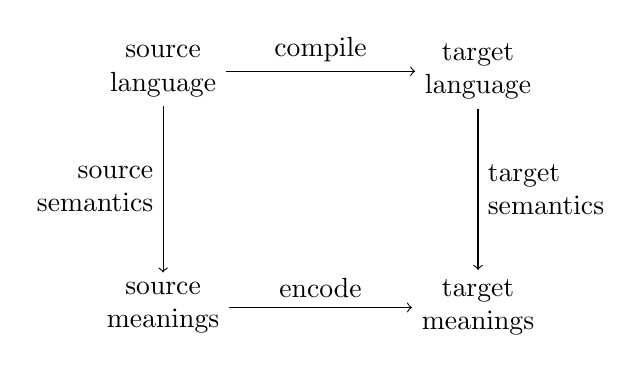
\begin{tikzpicture}
      \node[align=center] (S) at (0cm,3cm) {source\\language};
      \node[align=center] (T) at (4cm,3cm) {target\\language};
      \node[align=center] (M) at (0cm,0cm) {source\\meanings};
      \node[align=center] (U) at (4cm,0cm) {target\\meanings};
      
      \path (S) edge[->] node[align=center, above] {compile}           (T);
      \path (S) edge[->] node[align=right, left]   {source\\semantics} (M);
      \path (T) edge[->] node[align=left, right]   {target\\semantics} (U);
      \path (M) edge[->] node[align=center, above] {encode}            (U);
    \end{tikzpicture}
  \end{center}
  \caption{The commuting diagram used in the traditional approach to compiler verification}
  \label{commuting-diagram}
\end{figure}
Lockwood Morris\cite{morris1973} first observed that the commuting diagram approach was the usual approach to showing compiler correctness, though his version of the diagram had a decode function relating target meanings to source meanings.
Thatcher \emph{et al.}\cite{thatcher1979}, in extending Lockwood Morris' verification of a compiler, noticed that an encode function was more useful in reasoning and so included it in their diagram instead of the decode function.

The commuting diagram approach can be seen in some of the earliest work on compiler correctness, particularly McCarthy and Painter's paper from 1967\cite{mccarthy1967}.
McCarthy and Painter show the correctness of a compiler for a very simple expression language that targets a simple 4-instruction machine.
The source language consists only of constants, variables and addition to form expressions such as $(x + 3) + (y + z)$, and a function that evaluates these expressions to values under a particular variable binding forns the semantics of the source language.
The target machine consists of an acumulator register and a memory store with four instructions:
\begin{itemize}
  \item LI $\alpha$ --- which loads the immediate value $\alpha$ into the accumulator
  \item LOAD $x$ --- which loads a value from the memory location $x$ into the accumulator
  \item STO $x$ --- which stores the value in the accumulator in memory location $x$
  \item ADD $x$ --- which add the value at memory location $x$ to the value in the accumulator
\end{itemize}
The semantics of this target machine are defined by a function that takes an intial state and a list of instructions and outputs the final state.
McCarthy and Painter then define a compilation function from the source language to the target language.
The correctness of the compiler is defined by providing a function that puts the computed value of an expression into the accumulator of a machine state. 
It is then required that applying the function to the result of evaluating an expression is equivalent under a partial equality relation to the resultant state from compiling and running the expression.
The reason for the use of a partial equality is to ensure that any temporary variables introduced in compilation are ignored when comparing the machine states.
Though the use of partial equality and the equational way in which McCarthy and Painter state their definition of compiler correctness obscures it slightly, this can be seen as following the commuting diagram approach as shown in Figure~\ref{mccarthy1967-diagram}.
\begin{figure}
  \begin{center}
    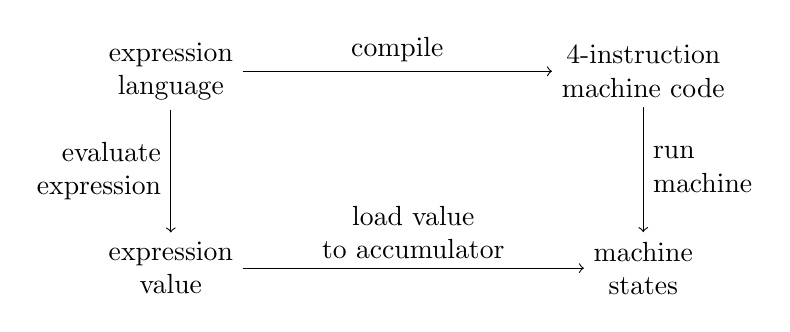
\begin{tikzpicture}
      \node[align=center] (S) at (0cm,2.5cm) {expression\\language};
      \node[align=center] (T) at (6cm,2.5cm) {4-instruction\\machine code};
      \node[align=center] (M) at (0cm,0cm)   {expression\\value};
      \node[align=center] (U) at (6cm,0cm)   {machine\\states};
      
      \path (S) edge[->] node[align=center, above] {compile}                    (T);
      \path (S) edge[->] node[align=right, left]   {evaluate\\expression}       (M);
      \path (T) edge[->] node[align=left, right]   {run\\machine}               (U);
      \path (M) edge[->] node[align=center, above] {load value\\to accumulator} (U);
    \end{tikzpicture}
  \end{center}
  \caption{A diagram showing how McCarthy and Painter's definition of compiler correctness follows the commuting diagram approach}
  \label{mccarthy1967-diagram}
\end{figure}

\section{Research Proposal}

\section{Preliminary Work}

\printbibliography
\end{document}